\documentclass[10pt,twocolumn,letterpaper]{article}
\usepackage{cvpr}
\usepackage{times}
\usepackage{epsfig}
\usepackage{graphicx}
\usepackage{amsmath}
\usepackage{amssymb}

% Include other packages here, before hyperref.

% If you comment hyperref and then uncomment it, you should delete
% egpaper.aux before re-running latex.  (Or just hit 'q' on the first latex
% run, let it finish, and you should be clear).
%\usepackage[pagebackref=true,breaklinks=true,letterpaper=true,colorlinks,bookmarks=false]{hyperref}

\cvprfinalcopy % *** Uncomment this line for the final submission

\def\cvprPaperID{****} % *** Enter the CVPR Paper ID here
\def\httilde{\mbox{\tt\raisebox{-.5ex}{\symbol{126}}}}

% Pages are numbered in submission mode, and unnumbered in camera-ready
\ifcvprfinal\pagestyle{empty}\fi
\begin{document}

%%%%%%%%% TITLE
\title{\LaTeX\ Author Guidelines for CVPR Proceedings}

\author{First Author\\
Institution1\\
Institution1 address\\
{\tt\small firstauthor@i1.org}
% For a paper whose authors are all at the same institution,
% omit the following lines up until the closing ``}''.
% Additional authors and addresses can be added with ``\and'',
% just like the second author.
% To save space, use either the email address or home page, not both
\and
Second Author\\
Institution2\\
First line of institution2 address\\
{\tt\small secondauthor@i2.org}
}

\maketitle
\thispagestyle{empty}

%%%%%%%%% ABSTRACT

\begin{abstract}
The main objective is to look at different classifiers which can be used for classifying images and analyze their performance.We then turn to \textit{Deep Learning} techniques which are good at finding patterns.We build a \textit{deep network} for classifying images and analyze its performance.
\end{abstract}
\section{Introduction}
The task is to predict the labels of images from the given categories buildings,cars,
flowers,faces,shoes. We here train the dataset with differnt classifiers like Neural Networks with backpropagation,Logistic Regression, Support Vector Machines.We further take our approach to apply DeepLearning methods and compare the results with our previous approaches.We will mainly look at:
 \begin{enumerate}
\item Sparse Autoencoders 
\item SelfTaught Learning 
\item Deep Networks 
\item Stacked Autoencoders 
 \end{enumerate}
\section{The Dataset}
The dataset consists of natural images taken from camera.The classes for the images are Buildings, Cars, Faces, Flowers and Shoes.Each image is 240 * 240 RGB image.We have 500 images for the training set and 1000 images for the test set.We have used SIFT algorithm to extract 240 feature from each of these images.For our deep learning tasks we will use samples from this raw images which are randomly picked.
\section{Training}
We describe here all the training approaches we have taken to train the classifier for multiclass object detection.We give brief description of all the training algorithms we have used.Finally we give the classification accuracy of this training algorithms on the test test we are using.
\subsection{Logistic Regression}
We will be using multiple one-vs-all logistic regression models to build a
multi-class classifier. Since there are 5
classes, we will need to train 5 separate logistic regression classifiers.
The cost function for logistic regression is:$$ J(\theta)=\frac{1}{m}\sum\limits_{i=1}^m[-y^{(i)}\log(h\theta(x^{(i)}))-(1-y^{(i)})\log(1-h\theta(x^{(i)}))] $$
Here,
$$ h\theta(x)=\frac{1}{1 + e^{-x}} $$
We have a training set of 500 examples.There are 240 feature vectors for each training set.Each feature represents a keypoint extracted from the image using SIFT algorithm.With these feature we train our clasifier using one vs all approach of code\footnote{www.github.com} Logistic Regression.After training we have a set of parameters which we use to predict the labels of the test set and determine its accuracy.
\subsection{Neural Nets with BackPropagation}
We use now Neural Networks which give a way of defining a complex,
non-linear form of hypotheses $h_{W,b}(x)$,with parameters $W,b$ that we can
fit to our data.To describe neural networks, we will begin by describing the simplest possible
neural network, one which comprises a single "neuron."
The "neuron" is a computational unit that takes as input $x_1, x_2, x_3$ (and a +1 intercept term), and
outputs $\textstyle h_{W,b}(x) = f(W^Tx) = f(\sum_{i=1}^3 W_{i}x_i +b)$, where $f : \Re \mapsto \Re$ is
called the 'activation function'.
$$ f(z) = \frac{1}{1+\exp(-z)} $$
A neural network is put together by hooking together many of our simple
"neurons," so that the output of a neuron can be the input of another.  For
example, here is a small neural network:
\begin{figure}[ht!]
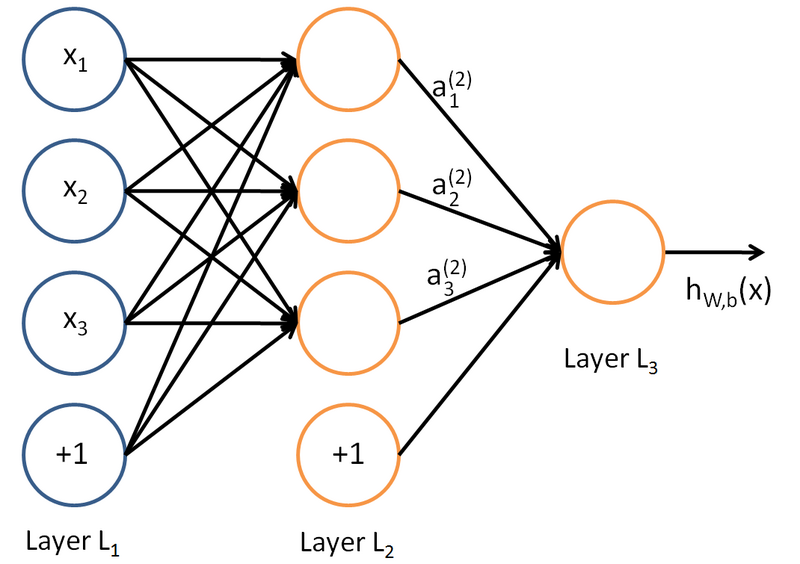
\includegraphics[width=8cm]{1.png}
\end{figure}
In this figure, we have used circles to also denote the inputs to the network.  The circles
labeled "+1" are called '''bias units''', and correspond to the intercept term.
The leftmost layer of the network is called the '''input layer''', and the
rightmost layer the '''output layer'''.The middle layer of nodes is called the '''hidden layer''', because its
values are not observed in the training set.  We also say that this example
neural network has 3 '''input units''' (not counting the bias unit), 3 
'''hidden units''', and 1 '''output unit'''.
We will let $n_l$ denote the number of layers in our network.
The neural network has parameters $(W,b) = (W^{(1)}, b^{(1)}, W^{(2)}, b^{(2)})$, where
$W^{(l)}_{ij}$ denote the parameter (or weight) associated with the connection
between unit $j$ in layer $l$, and unit $i$ in layer $l+1$.Also,$b^{(l)}_i$ is the bias associated with unit $i$ in layer $l+1$
Given a fixed setting of the parameters $W,b$,our neural network defines a hypothesis $h_{W,b}(x)$ that outputs a real number.
$$a_1^{(2)} = f(W_{11}^{(1)}x_1 + W_{12}^{(1)} x_2 + W_{13}^{(1)} x_3 + b_1^{(1)})$$
$$a_2^{(2)} = f(W_{21}^{(1)}x_1 + W_{22}^{(1)} x_2 + W_{23}^{(1)} x_3 + b_2^{(1)})$$
$$ a_3^{(2)} = f(W_{31}^{(1)}x_1 + W_{32}^{(1)} x_2 + W_{33}^{(1)} x_3 + b_3^{(1)})$$
$$h_{W,b}(x) = a_1^{(3)} =  f(W_{11}^{(2)}a_1^{(2)} + W_{12}^{(2)} a_2^{(2)} + W_{13}^{(2)} a_3^{(2)} + b_1^{(2)})$$
We call this step forward propagation.Neural networks can also have multiple output units.
Suppose we have a fixed training set $\{ (x^{(1)}, y^{(1)}), \ldots, (x^{(m)}, y^{(m)}) \}$ of $m$ training examples. We can train our neural network using batch gradient descent. In detail, for a single training example $(x,y)$, we define the cost function with respect to that single example to be:
$$ J(W,b; x,y) = \frac{1}{2} \left\| h_{W,b}(x) - y \right\|^2$$
This is a (one-half) squared-error cost function.The goal is to minimize $J(W,b)$ as a function of $W$ and $b$.We use backpropagation algorithm to minimize this cost function and get optimal set of weights to make predictions.
\subsection{Support Vector Machines}
A support vector machine constructs a hyperplane or set of hyperplanes in a high- or infinite-dimensional space, which can be used for classification, regression, or other tasks.Intuitively, a good separation is achieved by the hyperplane that has the largest distance to the nearest training data point of any class (so-called functional margin), since in general the larger the margin the lower the generalization error of the classifier.
Whereas the original problem may be stated in a finite dimensional space, it often happens that the sets to discriminate are not linearly separable in that space. For this reason, it was proposed that the original finite-dimensional space be mapped into a much higher-dimensional space, presumably making the separation easier in that space. To keep the computational load reasonable, the mappings used by SVM schemes are designed to ensure that dot products may be computed easily in terms of the variables in the original space, by defining them in terms of a kernel function $K(x,y)$ selected to suit the problem.The hyperplanes in the higher-dimensional space are defined as the set of points whose dot product with a vector in that space is constant. The vectors defining the hyperplanes can be chosen to be linear combinations with parameters $\alpha_i$ of images of feature vectors that occur in the data base. With this choice of a hyperplane, the points x in the feature space that are mapped into the hyperplane are defined by the relation: $\textstyle\sum_i \alpha_i K(x_i,x) = \mathrm{constant}$. Note that if K(x,y) becomes small as y grows further away from x, each term in the sum measures the degree of closeness of the test point x to the corresponding data base point $x_i$. In this way, the sum of kernels above can be used to measure the relative nearness of each test point to the data points originating in one or the other of the sets to be discriminated. Note the fact that the set of points x mapped into any hyperplane can be quite convoluted as a result, allowing much more complex discrimination between sets which are not convex at all in the original space.
Let us assume that we have $n$ labeled examples $(x_{1},y_{1}),\ldots,
(x_{n},y_{n})$ with labels $y_{i}\in \{1,-1\}$. We want to find the 
hyperplane $<w,x>+b = 0$ (i.e. with parameters $(w,b)$ ) satisfying
the followin three conditions:
\begin{enumerate}
  \item The scale of $(w,b)$ is fixed so that the plane is in canonical
        position w.r.t. $\{x_{1},\ldots,x_{n}\}$. i.e.,
\[ \min_{i\le n} | <w,x_{i}> + b | = 1 \]

  \item The plane with parameters $(w,b)$ separates the $+1$'s from the
        the $-1$'s. i.e., 
\[ y_{i} ( <w,x_{i}> + b ) \ge 0 \mbox{\ for all $i\le n$} \]

  \item The plane has maximum margin $\rho = 1/|w|$. i.e., minimum
        $|w|^{2}$.
\end{enumerate}
Of course there may not be a separating plane for the observed
data. Let us assume, for the time being, that the data is in fact
linearly separable and we'll take care of the general (more realistic)
case later.  


Clearly 1 and 2 combine into just one condition:
\[ y_{i}( <w,x_{i}> + b ) \ge 1 \mbox{\ for all $i\le n$}. \]
Thus, we want to solve the following optimization problem,

\[ \mbox{minimize\ } \frac{1}{2}|w|^{2} \]
over all $w\in R^{d}$ and $b\in R$ subject to,

\[ y_{i}( <w,x_{i}> + b ) -1 \ge 0 \mbox{\ for all $i\le n$}. \]

This is a very simple quadratic programming problem. There are readily
available algorithms of complexity $O(n^{3})$ that can be used for
solving this problem..
\subsection{Sparse Autoencoders}
Suppose we have only a set of unlabeled training examples $\textstyle \{x^{(1)}, x^{(2)}, x^{(3)}, \ldots\}$,
where $\textstyle x^{(i)} \in \Re^{n}$.An '''autoencoder''' neural network is an unsupervised learning algorithm that applies backpropagation,setting the target values to be equal to the inputs.  I.e., it uses $\textstyle y^{(i)} = x^{(i)}$
Here is an autoencoder:
\begin{figure}[ht!]
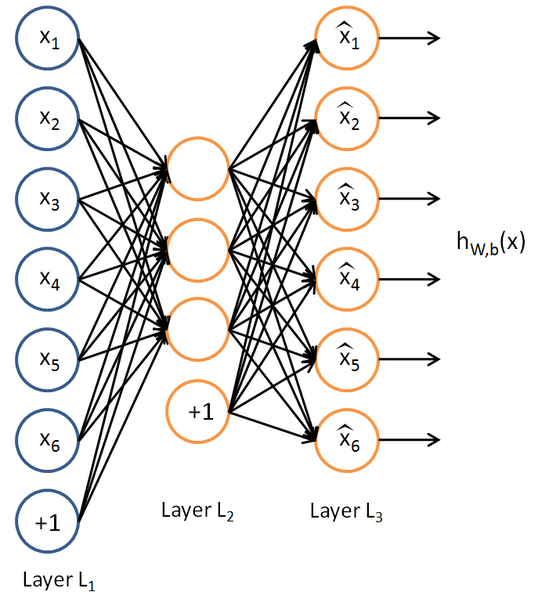
\includegraphics[width=8cm]{2.png}
\end{figure}
The autoencoder tries to learn a function $\textstyle h_{W,b}(x) \approx x$.In other
words, it is trying to learn an approximation to the identity function, so as
to output $\textstyle \hat{x}$ that is similar to $\textstyle x$.The identity function seems a
particularly trivial function to be trying to learn but by placing constraints
on the network, such as by limiting the number of hidden units, we can discover
interesting structure about the data.
Informally, we will think of a neuron as being "active" (or as "firing") if
its output value is close to 1, or as being "inactive" if its output value is
close to 0.  We would like to constrain the neurons to be inactive most of the
time. 
$\textstyle a^{(2)}_j$ denotes the activation of hidden unit $\textstyle j$ in the
autoencoder.  However, this notation doesn't make explicit what was the input $ x $
that led to that activation.Thus, we will write $\textstyle a^{(2)}_j(x)$ to denote the activation
of this hidden unit when the network is given a specific input $\textstyle x$.  Further, let
$$\hat\rho_j = \frac{1}{m} \sum_{i=1}^m \left[ a^{(2)}_j(x^{(i)}) \right]
$$ be the average activation of hidden unit $\textstyle j$
We would like to (approximately) enforce the constraint
$ \hat\rho_j = \rho,$
where $\textstyle \rho$ is a '''sparsity parameter''', typically a small value close to zero
.In other words, we would like the average activation
of each hidden neuron $\textstyle j$ to be close to 0.05 (say).  To satisfy this
constraint, the hidden unit's activations must mostly be near 0.
To achieve this, we will add an extra penalty term to our optimization objective that
penalizes $\textstyle \hat\rho_j$ deviating significantly from $\textstyle \rho$.We will choose the following:
$$
\sum_{j=1}^{s_2} \rho \log \frac{\rho}{\hat\rho_j} + (1-\rho) \log \frac{1-\rho}{1-\hat\rho_j}.
$$
\subsection{Deep Networks for Classification}
\subsection{Pre-Processing of Data}
\subsection{References}
\section{Final copy}

You must include your signed IEEE copyright release form when you submit
your finished paper. We MUST have this form before your paper can be
published in the proceedings.
\section{Final copy}

You must include your signed IEEE copyright release form when you submit
your finished paper. We MUST have this form before your paper can be
published in the proceedings.

Please direct any questions to the production editor in charge of these
proceedings at the IEEE Computer Society Press: Phone (714) 821-8380, or
Fax (714) 761-1784.

{\small
\bibliographystyle{plain}
\bibliography{test}
}

\end{document}
